\documentclass{article}
\usepackage[utf8]{inputenc}

\usepackage{latexsym}
\usepackage{float}
\usepackage[utf8]{inputenc}
\usepackage[catalan]{babel}
% \usepackage[english]{babel}
\usepackage{microtype}
\usepackage[hyphens]{url}
\usepackage{hyperref}
\usepackage{graphicx}
\usepackage{makeidx}
\usepackage{datetime}
\usepackage{multicol}
\usepackage{setspace}
\usepackage{enumerate}
\usepackage{booktabs}
\usepackage{listings}
\usepackage{color}
\usepackage{amsmath}
\usepackage{amssymb}
\usepackage[table,xcdraw]{xcolor}
\usepackage{graphicx}
\usepackage{listings}
\usepackage{hyperref}
\usepackage{vmargin}
\usepackage{wrapfig}
\usepackage{subfiles}
\usepackage{float}
\usepackage{amsmath}
\usepackage{amssymb}
\usepackage{tikz-cd}
\usepackage{multirow}
\usepackage{pgffor}
\usepackage{iflang}

%%%%%%%%%%%%%%%%%%%%%%%%%%%%%%%%%%%%%%%
%%%%%%%%%%%% UTIL COMMANDS %%%%%%%%%%%%  

\newcommand{\nc}{\newcommand}
\nc{\supindex}{\textsuperscript}

%%%%%%%%%%%%%%%%%%%%%%%%%%%%%%%%%%%%%%%
%%%%%%%%%%%%% CONFIG FILE %%%%%%%%%%%%%

\nc{\mytitle}{Anàlisis de fòrum anònim}
\nc{\mysubtitle}{Utilitzant Preferential Attachment sobre un pes inicial}
\nc{\authors}{Oriol Alàs Cercós}
\nc{\datetime}{30 d'octubre, 2020}
%15\supindex{th} of May, 2020}
\nc{\assignatura}{-}
\nc{\professorat}{Francesc Sebé}

% Per separar professors, utilitzar ','
% 	Ex: Maria, Joan, Pere

%%%%%%%%%%%%%%%%%%%%%%%%%%%%%%%%%%%%%%%
%%%%%%%%%%%%%  LANGUAGE   %%%%%%%%%%%%%

\newcommand{\tr}{\IfLanguageName{english}}

%%%%%%%%%%%%%%%%%%%%%%%%%%%%%%%%%%%%%%%
%%%%%%%%%%%%%%%%% MATH %%%%%%%%%%%%%%%%

\nc{\prob}[1]{P({#1})}
\nc{\probl}[2]{P({#1}|{#2})}

%%%%%%%%%%%%%%%%%%%%%%%%%%%%%%%%%%%%%%%
%%%%%%%%%%%%% TREE CREATOR %%%%%%%%%%%%

\setpapersize{A4}
\setmargins{2.5cm}  % margen izquierdo
{1.5cm}             % margen superior
{16.5cm}            % anchura del texto
{23.42cm}           % altura del texto
{10pt}              % altura de los encabezados
{1cm}               % espacio entre el texto y los encabezados
{0pt}               % altura del pie de página
{2cm}               % espaci\title{Determinització d'un autòmat finit}
\author{Oriol Alàs Cercós}
\date{29 d'Abril del 2019}

\def\contentsname{Índex}
\begin{document}
	

\begin{titlepage}
\begin{figure}[htb]
\begin{center}
	
\includegraphics[width=5cm]{imgs/UDL.png}
   	\vspace*{\stretch{1.0}}
   	\\
   	\medskip
   	\begin{center}
   		\noindent\rule{16.5cm}{0.4pt}
   		\medskip 
   		\\
      	\Huge\textbf{\mytitle}
      	\\\medskip 	\Large  \mysubtitle
      \\
      	
      	\noindent\rule{16.5cm}{0.4pt}
      	\\
      	\bigskip
      	\normalsize{\tr{Made by}{Realitzat per:}}
      	\\
      	\large\textit{\authors}
      	\\
      	\setlength{\parskip}{1em}
      	\normalsize{\tr{Delivery}{Data de lliurament:}}
      	\\
      	\large{\datetime}
   	\end{center}
   	\vspace*{\stretch{2.0}}
\end{center}
\end{figure}
\begin{flushright}
Universitat de Lleida
\\
Escola Politècnica Superior
\\
Grau en Enginyeria Informàtica
\\
\assignatura
\\
\medskip
\textbf{\tr{Professorate:}{Professorat:}}
\\
\foreach \n in \professorat{\n\\}
\end{flushright}
\thispagestyle{empty} 
\end{titlepage}
\tableofcontents
\thispagestyle{empty} 
%\newpage
\listoffigures
\listoftables
\thispagestyle{empty}
\newpage
\section{Introducció}
Per tal de veure la millora d'un Preferential Attachment amb certs pesos inicials per tal de bloquejar l'efecte inicial que donava prioritat a certs participants, s'ha realitzat una simulació amb 200 repeticiones per evitar casos outliers. No obstant això, certs paràmetres del problema han estat especificats per tal que totes les repeticions representin un sol cas general. Les dades especificades han estat:
\begin{itemize}
	\item Dades del sistema:
	\begin{itemize}	
		\item Nombre de participants: 200
		\item Ordre de l'anell: 6
	\end{itemize}
	\item Dades de la distribució
	\begin{itemize}
		\item Nombre màxim de missatges d'un participants: 15
		\item s: 1.4
	\end{itemize}
\end{itemize}
Per tal de buscar la relació entre el pes inicial i el pes de signatura, el rang d'aquestes variables ha estat:
\begin{itemize}
	\item pes inicial: [1,200]
	\item pes de signatura: [1, 4]
\end{itemize}
Com que es busca la relació entre el pes de 
\section{Anàlisis}
Per tal de realitzar l'anàlisis, s'ha buscat la mitjana i la mediana de la variable anonimitat per tal de buscar participants amb molta o poca prioritat (extrems). S'ha trobat més adhient buscar la variació entre els participants amb més prioritat, doncs aquests, influïran a haver més participants amb poca anonimitat.
\\
\\
S'ha trobat gràcies a la Figura \ref{fig:weight1}, s'ha vist que els millors valors inicials estan entre 10 i 35. No obstant això, en valors propers a 10 (i sobtadament en algun altre valor) encara es troben missatges sense anonimitat. La mostra de resultats es poden trobar a la Taula \ref{tab1}. No obstant això, la no anonimitat es troba en pesos inicials baixos, sent el màxim 22.
\begin{figure}[H]
	\centering
	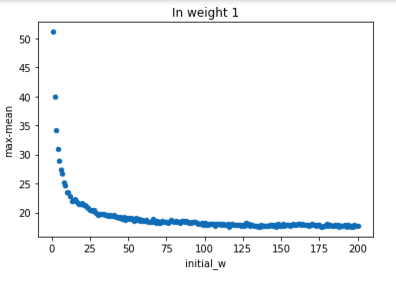
\includegraphics[width=7cm]{imgs/weight1.png}
	\label{fig:weight1}
	\caption{Gràfica de variació d'anonimitat entre el valor màxim i la mediana en cost de signatura=1.}
\end{figure}
\begin{figure}[H]
	\centering
	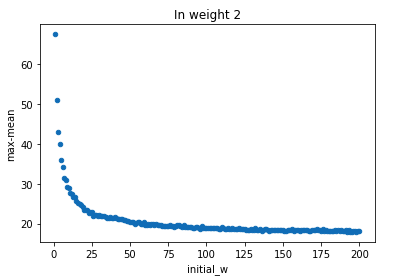
\includegraphics[width=7cm]{imgs/weight2.png}
	\label{fig:weight2}
	\caption{Gràfica de variació d'anonimitat entre el valor màxim i la mediana en cost de signatura=2.}
\end{figure}
\begin{figure}[H]
	\centering
	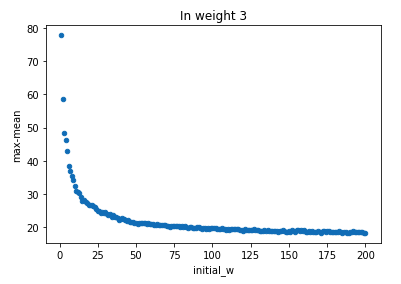
\includegraphics[width=7cm]{imgs/weight3.png}
	\label{fig:weight3}
	\caption{Gràfica de variació d'anonimitat entre el valor màxim i la mediana en cost de signatura=3.}
\end{figure}
\begin{figure}[H]
	\centering
	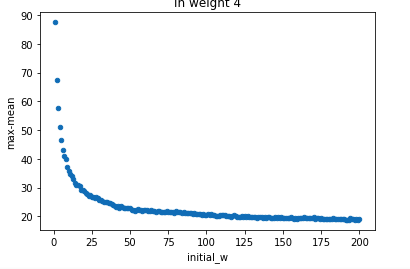
\includegraphics[width=7cm]{imgs/weight4.png}
	\label{fig:weight4}
	\caption{Gràfica de variació d'anonimitat entre el valor màxim i la mediana en cost de signatura=4.}
\end{figure}
\begin{table}[H]
	\centering
	\begin{tabular}{cc}
		initial weight & none-anonymity\\\hline
		8 & 0.010050 \\
		9 & 0.005025 \\
		10 & 0\\
		11& 0.010050\\
		12&0.005025 \\
		13&0.010050	\\
		14& 0.0 \\
		15&0.005025\\
		16& 0 \\
		17-20 & 0 \\
		21& 0 \\
		22 & 0.010050\\
		23& 0 \\
		24 - 200& 0 \\
	\end{tabular}
\label{tab1}
\caption{Taula de mitjana de no-anonimitat donat el pes inicial}
\end{table}
\section{Conclusió}
Seria interessant trobar una relació entre el pes inicial, pes per signatura, ordre de l'anell i nombre de participants. Per tal d'intentar eliminar la no-anonimitat de participants i assegurar privacitat, es podria realitzar una funció de cost.
\\
\\
Tot el codi es troba a \url{https://github.com/sergisi/glowing-dollop/}
\end{document}
